\chapter{Implementierung} % (fold)
\label{sec:implementierung}
Nachfolgend werden die Implementierung der verschiedenen APIs sowie die Grundprinzipien während der Implementierung beschrieben. Der Sourcecode der Implementierung ist unter der MIT Lizenz auf GitHub veröffentlicht. \citep{me}
\section{Grundprinzipien} % (fold)
\label{sec:prinzipien}
Im Rahmen der Implementierung der Anwendung wurden Grundprinzipien beachtet, die sowohl die Qualität als auch die Erweiterbarkeit der Anwendungen sicherstellten, wobei die Wahl der verwendeten Technologien sowie die Anwendung bewährter Praktiken im Vordergrund stand. Als Basis für die Entwicklung wurde Java JDK 17.0.10 Corretto gewählt, weil diese als Long-Term-Support-Version eine stabile und sichere Grundlage für die Entwicklung darstellt. Amazon Corretto bietet eine optimierte JVM, wodurch alle Softwarebestandteile auf jeder Plattform mit einer zertifizierten JAVA Virtual Machine lauffähig sind. Ergänzt wurde JDK durch Spring Boot Version 3.3.4, eine weit verbreitete Plattform für die Entwicklung von Webanwendungen und Microservices, die eine schnelle und einfache Konfiguration von Anwendungen ermöglicht sowie den Entwicklungsprozess durch das Automatisieren häufig auftretender Aufgaben vereinfacht, etwa der Konfiguration von Servern und Datenbankverbindungen. Als zentrales Konzept während der Implementierung diente die Verwendung von Dependency-Injection (DI). Diese Technik gewährleistet, dass die Abhängigkeiten zwischen den einzelnen Komponenten der Anwendung nicht hartkodiert sind, sondern zur Laufzeit durch den DI-Container von Spring injiziert werden. Dabei fördert DI die Entkopplung von Komponenten, was die Testbarkeit, Flexibilität und Wartbarkeit des Codes fördert. Weil der Code durch DI in unabhängige, umfangreich getestete Module unterteilt wird, lässt er sich leicht erweitern und an geänderte Anforderungen anpassen. Zudem trägt DI zur Lesbarkeit des Codes bei, weil Abhängigkeiten nicht explizit an anderen Stellen generiert werden müssen. Die Implementierung der Anwendung erfolgte weiter unter der Berücksichtigung von Best Practices, die die Qualität des Codes sicherstellen und eine effiziente, langfristige Wartung ermöglichen. Einen wesentlichen Aspekt bildete hierbei die Modularität der Lösung, wobei die Anwendung so strukturiert wurde, dass jede Komponente eine klare, abgegrenzte Verantwortung übernahm. Dies unterstützte nicht nur die Nachvollziehbarkeit des Codes, sondern erleichterte auch das Testen und die Erweiterung von Funktionalitäten. Bestehende Komponenten konnten so problemlos durch neue ersetzt oder erweitert werden, ohne die gesamte Anwendung zu beeinträchtigen.




% section prinzipien (end)

\section{Post-REST} % (fold)
\label{sec:postrest}
In dieser Arbeit steht ‚PostREST‘ für die PostgreSQL- REST-API, die eine Schnittstelle für den Zugriff auf eine PostgreSQL-Datenbank über HTTP-Anfragen bietet und mehrere Endpunkte implementiert, die in Abschnitt 5.2.1 der Arbeit definiert wurden und dafür verantwortlich sind, bestimmte Anfragen zu bearbeiten sowie entsprechende Antworten zurückzugeben. Als zentrale Komponente, die die korrekte Verarbeitung der Endpunkte sicherstellt, dient die Controller-Klasse (vgl Abb. 6.1), worin die Endpunkte integriert sind, wobei jeder Endpunkt mit seinen spezifischen Pfadvariablen und den Rückgabewerten versehen ist. Die Controller-Klasse übernimmt die Ausführung der richtigen Methoden, wenn eine Anfrage an einen bestimmten Endpunkt gestellt wird. Daneben beschreibt der PostrestController die konkrete Implementierung des Controllers, der die Geschäftslogik verarbeitet und den DBService aufruft, der das Interface IDBService implementiert, das wiederum die notwendigen Methoden für den Abruf von Daten aus den zugrunde liegenden Datenbanken definiert. Diese Methoden kapseln die Logik für den Datenbankzugriff und sind so gestaltet, dass sie von der Controller-Klasse verwendet werden können, um die korrekten Informationen zu erhalten. Die Kommunikation zwischen den verschiedenen Schichten der Anwendung erfolgt durch DI. Das bedeutet, dass die verschiedenen Komponenten nicht direkt in der Controller-Klasse erzeugt, sondern von außen in die Klasse injiziert werden, was in diesem Fall auf die Repositorys der verschiedenen Entitäten zutrifft. Diese Repositorys sind verantwortlich für den direkten Datenbankzugriff und beinhalten die notwendigen Methoden sowie SQL-Abfragen zum Abrufen und Verwalten der Daten in der Datenbank. Nachdem die Daten erfolgreich aus der Datenbank abgefragt wurden, werden sie durch die Hierarchie der Anwendung weitergegeben, wobei der PostrestController sicherstellt, dass die abgerufenen Daten ins gewünschte Format für die API-Antwort umgewandelt werden. Dies entspricht in diesem Fall dem JSON-Format, dass dem Nutzer der API als Antwort übermittelt wird. Diese Antwort enthält die über die API angeforderten Informationen des Nutzers.
\begin{figure}[H]
	\centering
	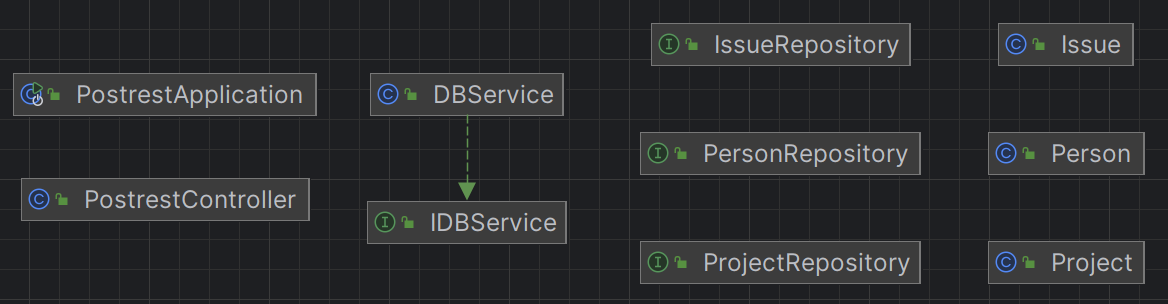
\includegraphics[scale=0.5]{Illustrations/postrest.png}
	\caption{PostREST-Java-Klassen}
\end{figure}
% section postrest (end)

\section{Post-Graph} % (fold)
\label{sec:postgraph}
Bei PostGraph handelt es sich um eine GraphQL-API, die mit einer PostgreSQL-Datenbank verbunden ist, wobei das Schema, das die Arbeitsweise der API beschreibt, wie bei GraphQL üblich, in der Datei schema.graphqls definiert wird. In dieser Datei sind die verschiedenen Datentypen sowie die möglichen Querys und Mutationen beschrieben, die zur Abfrage und Bearbeitung der Daten verwendet werden können. In den folgenden Abbildungen sind Bei- spiele für einen Typ, verschiedene Querys und eine Mutation entsprechend ihrer Definition in der schema.graphqls-Datei dargestellt:
\begin{figure}[H]
\begin{center}
\begin{BVerbatim}
type Issue{
    iid : ID!
    title : String
    createdAt : String
    state : String
    stateReason : String
}
\end{BVerbatim}
\end{center}
\caption{Typ aus der schema.graphqls-Datei}
\end{figure}
\begin{figure}[H]
\begin{center}
\begin{BVerbatim}
type Query{
    persons: [Person]
    person(id:ID!): Person
    projects: [Project]
    project(id:ID!) : Project
    issues : [Issue]
    issue(id: String): Issue
}
\end{BVerbatim}
\end{center}
\caption{Query aus der schema.graphqls-Datei}
\end{figure}
\begin{figure}[H]
\begin{center}
\begin{BVerbatim}

type Mutation {
    createIssue(input: IssueInput): Issue
}
\end{BVerbatim}
\end{center}
\caption{Mutation aus der schema.graphqls-Datei}
\end{figure}
\newpage
\noindent
Als zentrale Komponente für die Verarbeitung von Anfragen dient die Java-Klasse Query (vgl. Abb. 6.5), in der Methoden implementiert werden, die die Bearbeitung der An- fragen gemäß den Strukturen in der schema.graphqls-Datei ermöglichen. Diese Methoden greifen auf die Repositorys der Modellklassen zu, um Datenbankoperationen durchzuführen, wobei die Repositorys die erforderlichen Methoden und Logiken enthalten, um Daten in der PostgreSQL-Datenbank zu lesen oder zu ändern. Als wesentliches Merkmal von GraphQL gilt der Einsatz von Resolvern, die Felder verarbeiten, die auf Daten aus anderen Quellen oder Datenbanken basieren. Resolver stellen sicher, dass die relevanten Daten korrekt abgerufen und in der gewünschten Struktur zurückgegeben werden. Die Repositorys werden in die benötigten Klassen injiziert, sodass sie nicht direkt innerhalb der Anwendung erstellt werden müssen. Nach erfolgreicher Bearbeitung einer Anfrage liefert die GraphQL-API die Daten im vorgegebenen GraphQL-Format an den Nutzer zurück, was eine flexible und leistungsfähige Schnittstelle zur Abfrage und Manipulation der Daten in der zugrunde liegenden PostgreSQL-Datenbank gewährleistet.
\begin{figure}[H]
	\centering
	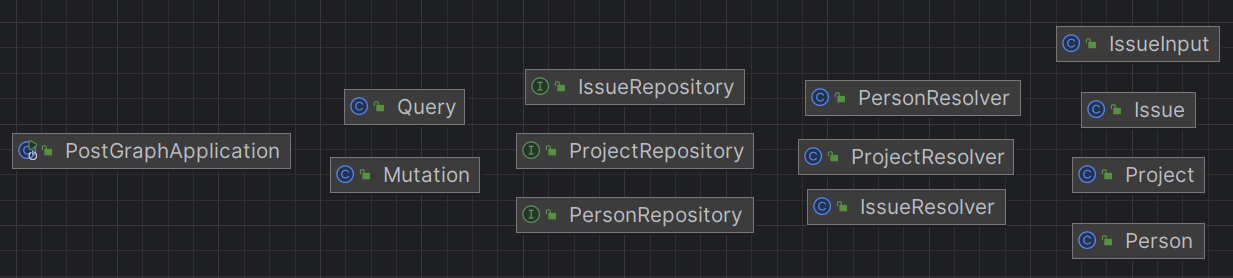
\includegraphics[scale=0.5]{Illustrations/postgraph.png}
	\caption{ PostGraph-Java-Klassen}
\end{figure}
% section postgraph (end)

\section{Neo4REST} % (fold)
\label{sec:neo4rest}
Neo4REST beschreibt eine REST-API, die den Zugriff auf eine Neo4j-Datenbank ermöglicht. Analog zur Struktur von PostREST bietet Neo4REST mehrere Endpunkte, die zur Bearbeitung spezifischer Anfragen und zur Rückgabe der entsprechenden Antworten dienen; Details dieser Endpunkte sind in Abschnitt 5.2.2 definiert. Die Verarbeitung der Endpunkte wird durch die zentrale Controller-Klasse sichergestellt (vgl. Abb. 6.7), in der wie bei PostREST die spezifischen Pfadvariablen, Parameter und Rückgabewerte der Endpunkte definiert sind. Durch die Controller-Klasse werden die passenden Methoden aufgerufen, sobald eine Anfrage an einen der Endpunkte gestellt wird, wobei der Neo4RestController die Geschäftslogik übernimmt und datenbankbezogene Aufgaben an den DBService delegiert, der das Interface IDBService implementiert. Dieses Interface definiert die für den Zugriff auf die Neo4j-Datenbank erforderlichen Methoden, wobei die Umsetzung der konkreten Abfragen über Repositorys erfolgt, die für die Durchführung der Cypher-Abfragen zuständig sind. Diese Repositorys abstrahieren den Datenbankzugriff und bieten wiederverwendbare Methoden, um auf die in Neo4j gespeicherten Daten zuzugreifen oder sie zu ändern. Wie bei PostREST werden die in der Datenbank abgefragten Informationen, durch die Schichten der Anwendung weitergeleitet und im Controller ins JSON-Format umgewandelt, bevor sie als API-Antwort zurückgegeben werden. So stellt Neo4REST sicher, dass der Nutzer die angeforderten Informationen oder den Status einer Operation im passenden Format erhält.
\begin{figure}[H]
	\centering
	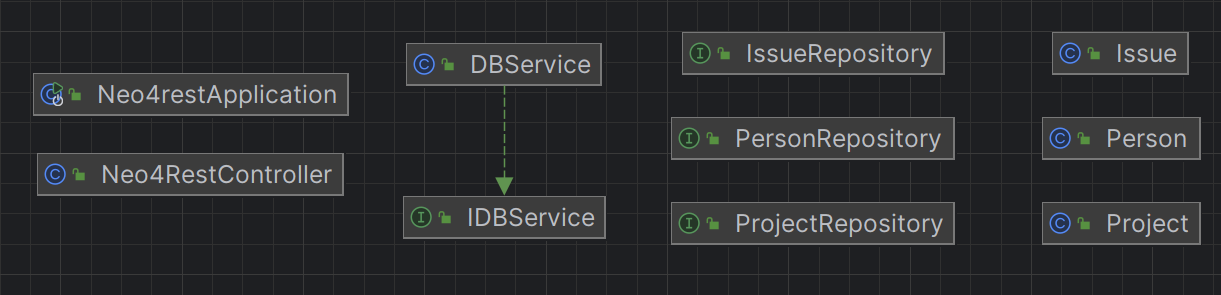
\includegraphics[scale=0.5]{Illustrations/neo4rest.png}
	\caption{Neo4REST-Java-Klassen }
\end{figure}
% section neo4rest (end)

\section{Neo4Graph} % (fold)
\label{sec:neo4graph}
Die Neo4Graph-API stellt eine GraphQL-API dar, die mit einer Neo4j-Datenbank verbunden ist, wobei das bereits in Bezug auf die PostGraph-API beschriebene Schema bei Neo4Graph auf ähnliche Weise implementiert wird: Wie bei PostGraph kommen Cypher-Abfragen zum Einsatz, um mit der Neo4j-Datenbank zu interagieren. Die Methoden nutzen die Neo4j- Clientbibliothek, um Knoten und Kanten effizient zu durchsuchen sowie Datenbankoperationen durchzuführen. Ein weiteres gemeinsames Merkmal beider APIs stellt der Einsatz von Resolvern dar, die bei Neo4Graph ebenfalls zur Bearbeitung von Feldern verwendet werden, die auf Beziehungen oder aggregierten Daten im Graphen basieren. Resolver sorgen dafür, dass die benötigten Daten korrekt abgerufen und in der gewünschten Struktur zurückgegeben werden. Nach der Bearbeitung einer Anfrage liefert die GraphQL-API die Daten im standardisierten GraphQL-Format an den Nutzer, was eine konsistente und leistungsfähige Schnittstelle zur Abfrage sowie Bearbeitung der Daten in der Neo4j-Datenbank sicherstellt.

\begin{figure}[H]
	\centering
	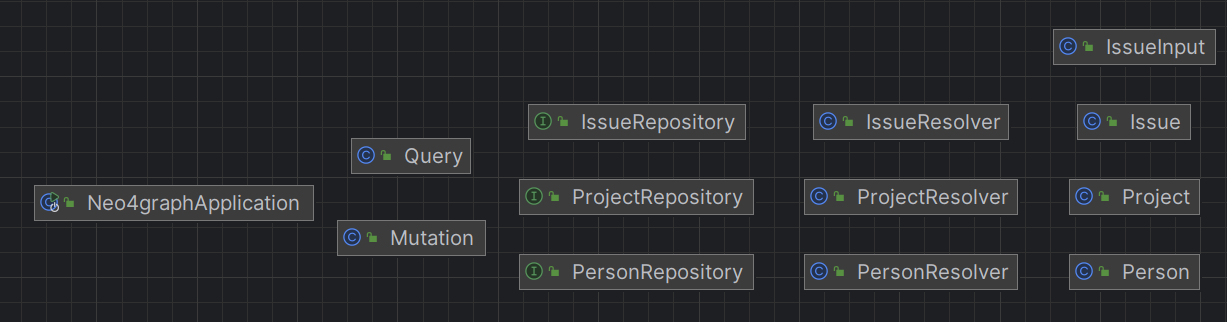
\includegraphics[scale=0.5]{Illustrations/neo4graph.png}
	\caption{Neo4Graph-Java-Klassen}
\end{figure}
% section neo4graph (end)
\section{API-Response-Test} % (fold)
\label{sec:test}
Für die Ermöglichung von API-Anfragen von einem entfernten System aus wurde eine Anwendung entwickelt, die für jeden Endpunkt eine Methode enthält (vgl. Abb. 6.8), die jeweils hundert Abfragen in einer Schleife ausführt. Falls für eine Abfrage eine ID erforderlich ist, wird diese mithilfe der Klasse Random aus java.util.Random generiert. Die Abfragen für den parametrisierten Endpunkt werden mit den Joins von 0 bis 3 und den Ergebnistupeln 1, 100, 1000, 10 000 sowie 100 000 durchgeführt, wobei die Abfragezeit ermittelt wird, indem die aktuelle Systemzeit in Millisekunden unmittelbar vor der Ausführung der Abfrage erfasst und von der Zeit nach Abschluss der Abfrage abgezogen wird.
\begin{figure}[H]
	\centering
	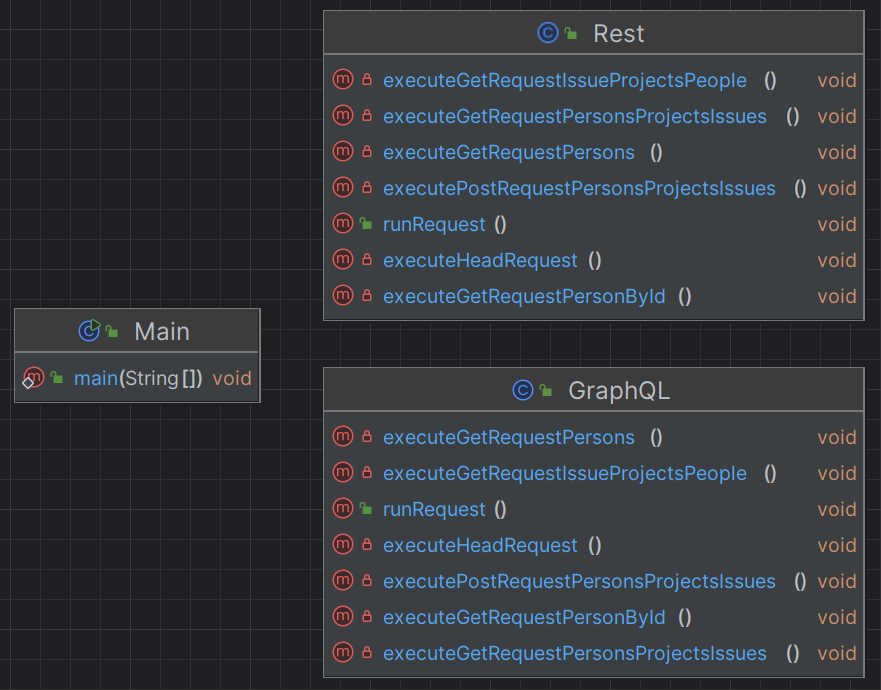
\includegraphics[scale=0.5]{Illustrations/apiresponsetest.png}
	\caption{Java Klassen Neo4Graph}
\end{figure}
% section test (end)
% chapter implementierung (end)